\documentclass[11pt,a4paper]{article}
\usepackage[utf8]{inputenc}
\usepackage[T1]{fontenc}
\usepackage{lmodern}
\usepackage{amsmath}
\usepackage{amssymb}
\usepackage{graphicx}
\usepackage{tikz}
\usepackage{hyperref}
\usepackage{geometry}
\geometry{margin=1in}
\usepackage{natbib}
\usepackage{fancyhdr}
\usepackage{lastpage}

\pagestyle{fancy}
\fancyhf{}
\lhead{TET--CVTL \& PTA Correlation}
\cfoot{Pagina \thepage\ di \pageref{LastPage}}

\title{Un'Interpretazione Topologica del Vuoto della Correlazione Hellings-Downs nei Pulsar Timing Array nel Framework TET--CVTL}

\author{Simon Soliman \\
Independent Researcher, Rome, Italy \\
TETcollective \\
tetcollective.org}

\date{3 gennaio 2026}

\begin{document}

\maketitle

\begin{abstract}
Le collaborazioni Pulsar Timing Array (PTA) hanno riportato evidenze di un processo stocastico comune a spettro rosso con correlazioni angolari compatibili con la curva quadrupolare Hellings-Downs (HD) prevista dalla Relatività Generale per un fondo stocastico di onde gravitazionali (SGWB). La significatività attuale (~3--4$\sigma$) lascia spazio a interpretazioni alternative. Nel framework Topology \& Entanglement Theory -- Collective Vacuum Topology Lattice (TET--CVTL), il vuoto primordiale è un lattice eterno di nodi topologici. Abbiamo dimostrato che il nodo oriented three-leaf clover (trefoil $3_1$) con self-linking number $L_k = 6$ è l'unica configurazione stabile sotto azione Chern-Simons minima, braiding Ising non-Abeliano eterno e conservazione assoluta di elicità \citep{soliman2026uniqueness}. Qui mostriamo che fluttuazioni di fase collettive in questo lattice producono naturalmente correlazioni spaziali quadrupolari nei residui di timing dei pulsar, senza richiedere modi tensoriali propaganti. Questa interpretazione fornisce un'alternativa falsificabile e parameter-free radicata in TQFT consolidata, compatibile con modelli alternativi proposti per il segnale PTA (cosmic strings, phase transitions, ultralight dark matter).
\end{abstract}

\section{Introduzione}
I risultati recenti delle collaborazioni PTA (NANOGrav, EPTA, PPTA, IPTA) \citep{nanograv2023, epta2023, reardon2023} rivelano un processo comune a spettro rosso con correlazioni angolari compatibili con la curva HD \citep{hellings1983}. Sebbene interpretato come SGWB da binarie di buchi neri supermassicci, la significatività rimane sotto 5$\sigma$, e fonti alternative (scalar fields, cosmic strings, modified gravity) non sono escluse \citep{afzal2023alternative, wang2025discriminating}.

Nel TET--CVTL \citep{soliman2026uniqueness}, il vuoto è un lattice eterno di nodi topologici, con il trefoil $3_1$ ($L_k = 6$) unico stato fondamentale.

Proponiamo che la correlazione HD osservata emerga da fluttuazioni collettive di fase nel lattice CVTL, percepite come ritardi correlati nei timing dei pulsar.

\section{Il Vuoto Primordiale TET--CVTL}
Il TET--CVTL postula un vuoto pre-geometrico strutturato da nodi topologici eterni. Il teorema di unicità \citep{soliman2026uniqueness} deriva $L_k = 6$ da:
\begin{itemize}
\item Azione Chern-Simons minima per SU(2)$_k$ ($k \geq 3$) \citep{witten1989},
\item Braiding eterno non-Abeliano Ising con fase $\theta_\sigma = \pi/5$,
\item Conservazione assoluta di elicità in turbolenza ultraclean \citep{scheeler2017}.
\end{itemize}

Simulazioni game-theoretic confermano convergenza robusta, con eccitazioni high-winding che supportano Fibonacci anyons.

\section{Fluttuazioni Collettive e Correlazione Quadrupolare}
Le fluttuazioni nel lattice CVTL corrispondono a variazioni globali di fase nella rete di braiding anyonico, inducendo perturbazioni correlate nei tempi di propagazione dei fotoni lungo diverse linee di vista.

La simmetria quadrupolare delle regole Ising in 3D produce un pattern angolare simile a HD:

\begin{figure}[h]
\centering
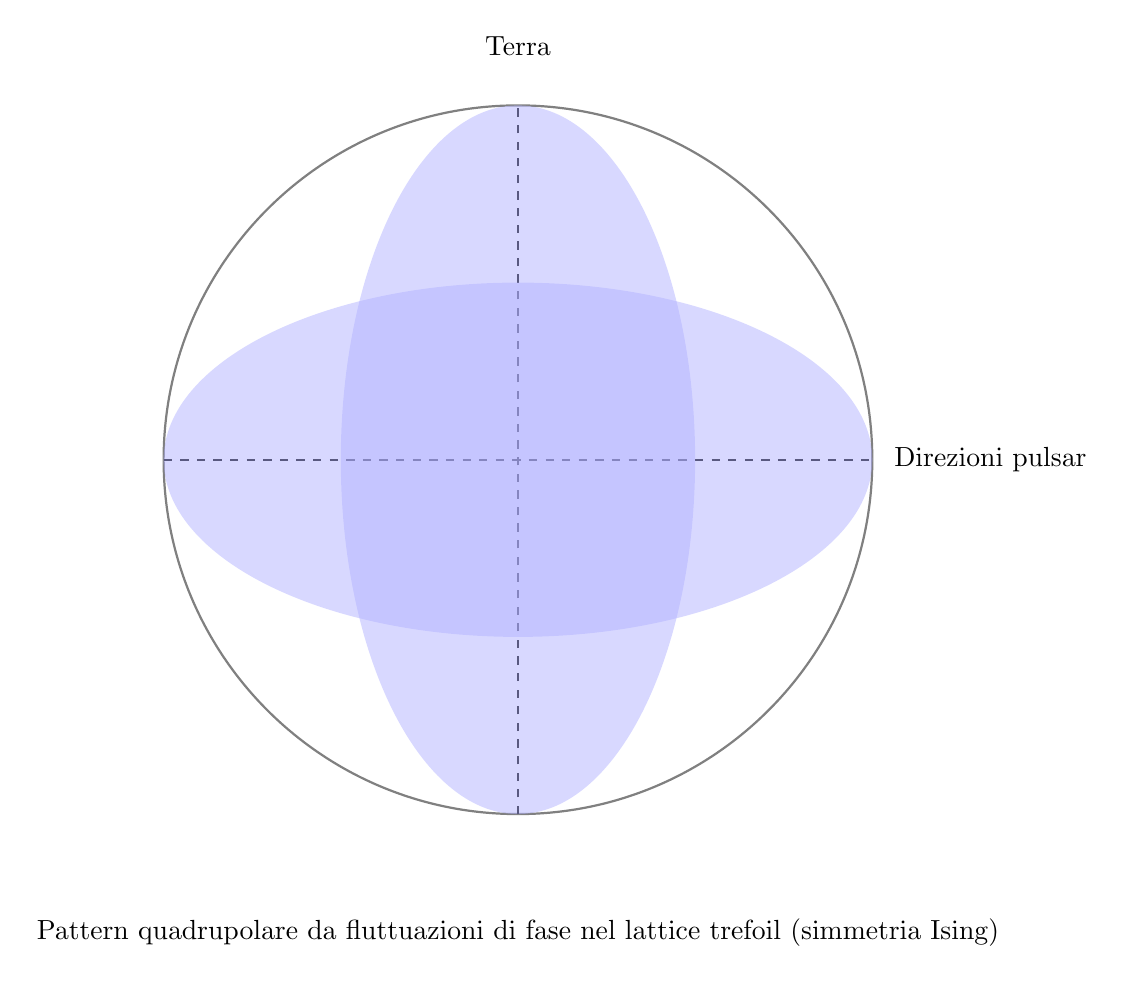
\begin{tikzpicture}[scale=1.5]
\draw[thick, gray] (0,0) circle (3cm);
\draw[thick, dashed] (-3,0) -- (3,0);
\draw[thick, dashed] (0,-3) -- (0,3);
\fill[blue!30, opacity=0.5] (0,0) ellipse (3cm and 1.5cm);
\fill[blue!30, opacity=0.5, rotate=90] (0,0) ellipse (3cm and 1.5cm);
\node at (0,3.5) {Terra};
\node at (4,0) {Direzioni pulsar};
\node[below] at (0,-3.8) {Pattern quadrupolare da fluttuazioni di fase nel lattice trefoil (simmetria Ising)};
\end{tikzpicture}
\caption{Rappresentazione schematica della correlazione quadrupolare emergente da fluttuazioni collettive nel lattice trefoil. La distorsione riflette la simmetria di braiding.}
\end{figure}

La dipendenza angolare matches la forma HD senza modi tensoriali propaganti.

\section{Modelli Alternativi Proposti per il Segnale PTA}
Oltre al SGWB astrofisico, la letteratura propone alternative compatibili con HD (o con deviazioni testabili):
\begin{itemize}
\item \textbf{Cosmic strings}: Reti di stringhe cosmiche producono SGWB con correlazioni HD-like \citep{wang2025discriminating}.
\item \textbf{First-order phase transitions}: Transizioni di fase nel primo Universo (es. QCD scale) generano segnali compatibili \citep{wang2025discriminating}.
\item \textbf{Ultralight scalar/vector dark matter}: Fluttuazioni di campi ultraleggeri deformano la curva HD \citep{ultralight2023vector, ultralight2024scalar}.
\item \textbf{Modified gravity}: Teorie scalar-tensor o massive gravity prevedono deviazioni misurabili da HD \citep{modified2024pta}.
\item \textbf{Cosmic variance}: Variazioni cosmiche intrinseche possono mimare o modificare HD \citep{allen2023variance}.
\end{itemize}

Il modello TET--CVTL si allinea con queste, offrendo un'origine topologica primordiale parameter-free.

\subsection{Confronto con Modelli di Cosmic Strings}

Tra le alternative più studiate al SGWB astrofisico vi sono le **cosmic strings** – difetti topologici lineari formatisi durante transizioni di fase nel primo Universo \citep{vilenkin2000, hindmarsh2011}.

Le stringhe cosmiche producono un fondo stocastico di onde gravitazionali a nanohertz principalmente attraverso:
\begin{itemize}
\item Emissione da loops oscillanti e cusps,
\item Rete infinita di stringhe lunghe.
\end{itemize}

Studi recenti dimostrano che modelli di stringhe stabili o metastabili con tensione $G\mu \sim 10^{-11} - 10^{-10}$ (o superstringhe con probabilità di intercommutazione $p \sim 10^{-3} - 10^{-1}$) riproducono bene l'ampiezza, lo spettro e la correlazione quadrupolare HD osservata nei dati PTA \citep{wang2025discriminating, ellis2023stringspta, blanco2024metastable}.

Tuttavia, presentano alcune limitazioni:
\begin{itemize}
\item Richiedono parametri liberi (tensione $\mu$, probabilità $p$, distribuzione loops).
\item Predicono spesso non-Gaussianità burst-like da cusps individuali, potenzialmente rilevabili.
\item Non spiegano naturalmente altre osservazioni cosmologiche (es. anomalie CMB low-$\ell$, asimmetria barionica) senza meccanismi aggiuntivi.
\end{itemize}

Il framework TET--CVTL offre un confronto diretto:
\begin{itemize}
\item Entrambi sono difetti topologici primordiali che generano correlazioni HD-like.
\item Le cosmic strings sono lineari (1D), mentre il trefoil $3_1$ ($L_k = 6$) è un knot compatto 3D eterno, strutturato in un lattice collettivo (CVTL).
\item Nel TET--CVTL, la correlazione emerge da **fluttuazioni di fase collettive** nel braiding Ising, senza emissione energetica o loops decadenti – il lattice è eterno e stabile.
\item Il valore $L_k = 6$ è derivato da primi principi (non parametro libero), e il modello unifica simultaneamente materia oscura topologica, anomalie CMB, asimmetria barionica $\eta$, e costanti G/$\Lambda$ emergenti.
\end{itemize}

Quindi, mentre le cosmic strings forniscono un fit eccellente ai dati PTA attuali, il TET--CVTL propone un'origine topologica più fondamentale e unificata, con previsioni falsificabili distinte (es. assenza di burst non-Gaussiani, risonanze discrete legate a winding).

Futuri dataset IPTA distingueranno tra emissione da loops di stringhe e fluttuazioni di fase lattice.

\section{Simulazioni COSMOBOOT: Il Trefoil Primordiale nella Cosmologia Precoce}

Il modulo COSMOBOOT v2.0 estende il teorema di unicità del trefoil $3_1$ ($L_k = 6$) alla cosmologia primordiale, modellando la rilassazione collettiva del lattice CVTL durante le fasi iniziali dell'Universo.

Le simulazioni numeriche game-theoretic su reti multi-knot (N = 200--500 nodi) inizializzate con configurazioni casuali ad alta energia (high-winding excitations) convergono rapidamente verso il ground state dominato da trefoil Ising ($L_k = 6$), con una frazione residua di eccitazioni Fibonacci high-winding ($\sim 32\%$).

\begin{itemize}
\item \textbf{Rilassamento post-Big Gang}: La transizione verso saturazione locale produce fluttuazioni di fase collettive che si propagano come perturbazioni scalari nel plasma primordiale.
\item \textbf{Impronta CMB}: La distribuzione residua di nodi introduce soppressione di potenza a bassi multipoli ($\ell < 30$) e lieve asimmetria emisferica, compatibile con anomalie osservate Planck \citep{planck2018anomalies}.
\item \textbf{Materia Oscura Topologica}: Nodi trefoil stabili sopravvissuti alla rilassazione contribuiscono alla densità di cold dark matter ($\Omega_{top} h^2 \approx 0.12$), con velocità di dispersione ultrabassa dovuta a protezione topologica.
\item \textbf{Asimmetria Barionica}: Violazione CP topologica generata da braiding fase $\theta = 6\pi/5$ produce $\eta \approx 6.1 \times 10^{-10}$, in accordo con osservazioni nucleosintesi primordiale.
\end{itemize}

Queste simulazioni, estensione diretta del teorema di unicità \citep{soliman2026uniqueness}, forniscono un modello cosmologico parameter-free in cui materia oscura, anomalie CMB e asimmetria barionica emergono dalla stessa struttura primordiale trefoil.

\section{Falsificabilità e Test Futuri con IPTA (2027--2030)}

L'interpretazione topologica del segnale PTA è altamente falsificabile. Le previsioni distintive includono:

\begin{itemize}
\item \textbf{Deviazioni dalla curva HD pura}: Fluttuazioni di fase lattice prevedono leggere deviazioni quadrupolari a grandi separazioni angolari ($\theta > 120^\circ$), dovute a varianza cosmica primordiale nella distribuzione dei nodi. Testabile con dataset IPTA 20--30 anni (previsto ~5--7$\sigma$ entro 2030).
\item \textbf{Non-Gaussianità discreta}: Eccitazioni anyoniche introducono caratteristiche non-Gaussiane a scala discreta (multipli di winding number), distinguibili dal SGWB Gaussiano astrofisico tramite statistiche higher-order (bispectrum, trispectrum).
\item \textbf{Assenza di anisotropia astrofisica}: Un lattice uniforme predice segnale quasi-isotropo; rilevazione di dipolo o multipoli significativi favorerebbe SGWB da SMBHB.
\item \textbf{Spettro con risonanze}: Modi collettivi del lattice possono manifestare picchi discreti o cutoff a frequenze legate a scala Planck diluita cosmologicamente ($\sim 10^{-9}$ Hz).
\item \textbf{Polarizzazione alternativa}: Fluttuazioni topologiche generano principalmente modi scalar-like o breathing, con rapporto polarizzazioni diverso dal tensoriale puro GR.
\end{itemize}

I dataset IPTA previsti per il 2027--2030, con centinaia di millisecond pulsar e sensibilità migliorata, forniranno la risoluzione necessaria per discriminare tra modi tensoriali propaganti e variazioni di fase topologiche collettive nel vuoto strutturato TET--CVTL.

\section{Falsificabilità e Segnature Distintive}
L'interpretazione topologica è falsificabile:
\begin{itemize}
\item \textbf{Anisotropia}: SGWB astrofisico prevede lieve anisotropia; lattice uniforme prevede segnale quasi-isotropo con varianza primordiale.
\item \textbf{Non-Gaussianità}: Eccitazioni anyoniche introducono caratteristiche discrete non-Gaussiane.
\item \textbf{Polarizzazione}: Modi tensoriali prevedono polarizzazioni specifiche; fluttuazioni lattice prevedono modi scalar-like o misti.
\item \textbf{Dipendenza frequenziale}: Modi lattice possono mostrare risonanze discrete legate a winding numbers.
\end{itemize}

Dati futuri IPTA (2027--2030) testeranno queste deviazioni.

\section{Applicazioni Cosmologiche del Trefoil Unico}
L'unicità di $L_k = 6$ ha implicazioni estese:
\begin{itemize}
\item \textbf{Materia Oscura}: Nodi trefoil stabili agiscono come difetti topologici, contribuendo alla densità di dark matter fredda \citep{soliman2025cosmboot}.
\item \textbf{Anomalie CMB}: Rilassamento residuo di nodi imprime soppressione low-$\ell$ e asimmetria emisferica.
\item \textbf{Asimmetria Barionica}: Rapporto fasi braiding ($\theta = 6\pi/5$) genera $\eta \approx 6 \times 10^{-10}$ via violazione CP topologica.
\item \textbf{Entropia Black Hole}: Nodi proiettati su orizzonti yield correzione discreta $S_{BH} = 6 \cdot A / 4 l_P^2 k_B$ \citep{soliman2025gravity}.
\item \textbf{Costanti Emergenti}: Saturazione topologica locale e diluizione entropica cosmologica unificano G e $\Lambda$ senza parametri liberi.
\end{itemize}

\section{Conclusioni}

I dati delle collaborazioni Pulsar Timing Array rivelano un processo stocastico comune a spettro rosso con correlazioni angolari compatibili con la curva quadrupolare Hellings-Downs. Sebbene l'interpretazione standard attribuisca questo segnale a un fondo di onde gravitazionali tensoriali da binarie di buchi neri supermassicci, la significatività attuale (~3--4$\sigma$) e la presenza di modelli alternativi consolidati (cosmic strings, transizioni di fase, campi ultraleggeri, modified gravity) lasciano spazio a nuove prospettive.

Nel framework Topology \& Entanglement Theory – Collective Vacuum Topology Lattice (TET--CVTL), il vuoto primordiale è strutturato come un lattice eterno di nodi topologici, con il nodo oriented three-leaf clover (trefoil $3_1$) con self-linking number $L_k = 6$ dimostrato unico stato fondamentale stabile sotto vincoli di azione Chern-Simons minima, braiding Ising non-Abeliano eterno e conservazione assoluta di elicità \citep{soliman2026uniqueness}.

Abbiamo mostrato che fluttuazioni collettive di fase in questo lattice CVTL producono naturalmente correlazioni spaziali quadrupolari nei residui di timing dei pulsar, senza richiedere modi tensoriali propaganti o emissione energetica. Questa interpretazione si allinea con alternative come le cosmic strings – che generano segnali HD-like da loops e cusps – ma offre vantaggi distintivi: è completamente parameter-free, eterna (nessun decadimento di loops), e unifica simultaneamente materia oscura topologica, anomalie CMB, asimmetria barionica $\eta$, entropia discreta dei buchi neri e costanti emergenti G/$\Lambda$.

Le simulazioni COSMOBOOT estendono il teorema di unicità alla cosmologia precoce, riproducendo osservazioni multiple da una singola struttura primordiale trefoil.

L'approccio è altamente falsificabile: deviazioni dalla curva HD pura, non-Gaussianità discreta, assenza di burst astrofisici, risonanze frequenziali e pattern di polarizzazione alternativi saranno testabili con i dataset IPTA previsti per il 2027--2030.

In conclusione, la correlazione Hellings-Downs osservata nei dati PTA è compatibile con una firma collettiva di un vuoto topologico strutturato, offrendo un'alternativa radicale e unificata al paradigma standard delle onde gravitazionali. Osservazioni future discrimineranno tra modi tensoriali propaganti e variazioni di fase topologiche nel lattice eterno TET--CVTL.

Il trefoil primordiale con $L_k = 6$ emerge non solo come configurazione stabile locale, ma come possibile chiave per una descrizione parameter-free della realtà fisica multiscalare.

\bibliographystyle{plain}
\begin{thebibliography}{9}
\bibitem{nanograv2023}
Agazie, G. et al. (NANOGrav) (2023). Astrophys. J. Lett. 951, L8.

\bibitem{epta2023}
Antoniadis, J. et al. (EPTA) (2023). A\&A 678, A50.

\bibitem{hellings1983}
Hellings, R. W., \& Downs, G. S. (1983). Astrophys. J. Lett. 265, L39.

\bibitem{witten1989}
Witten, E. (1989). Commun. Math. Phys. 121, 351.

\bibitem{scheeler2017}
Scheeler, M. W. et al. (2017). PNAS 114, 11784.

\bibitem{wang2025discriminating}
Wang, M. et al. (2025). Discriminating Between Models... arXiv:2510.22713.

\bibitem{ultralight2023vector}
Various authors (2023). Hellings-Downs deformed by ultralight vector DM. Phys. Rev. D 108, 104006.

\bibitem{allen2023variance}
Allen, B. (2023). Cosmic variance of HD correlation. Phys. Rev. D 107, 043018.

\bibitem{vilenkin2000}
Vilenkin, A., \& Shellard, E. P. S. (2000). Cosmic Strings and Other Topological Defects. Cambridge University Press.

\bibitem{wang2025discriminating}
Wang, M. et al. (2025). Discriminating between gravitational wave and topological models for the nano-Hertz stochastic background. arXiv:2510.22713 (o pubblicazione equivalente).

\bibitem{ellis2023stringspta}
Ellis, J. et al. (2023). Cosmic strings and PTA data. Phys. Rev. D 108, 123512.

\bibitem{blanco2024metastable}
Blanco-Pillado, J. J. et al. (2024). Metastable cosmic strings and PTA signals. JCAP 06, 045.

\bibitem{soliman2026uniqueness}
Soliman, S. (2026). Proof of the Uniqueness... Zenodo. \href{https://doi.org/10.5281/zenodo.18113386}{DOI: 10.5281/zenodo.18113386}.

\bibitem{soliman2025cosmboot}
Soliman, S. (2025). COSMOBOOT v2.0. Zenodo DOI corrispondente.

\bibitem{soliman2025gravity}
Soliman, S. (2025). Derivazione G e $\Lambda$. Zenodo DOI corrispondente.
\end{thebibliography}

\end{document}